
\documentclass[11pt]{amsbook}

\usepackage{../HBSuerDemir}	% ------------------------


\begin{document}

% ++++++++++++++++++++++++++++++++++++++
\hPage{b1p2/335}
% ++++++++++++++++++++++++++++++++++++++
\begin{enumerate}
	\setcounter{enumi}{73}

	\item Sketch the following loci of points in z-plane:\\
	a) $\frac{Re\ z}{|z - 1|}$ = 1,  b) $\frac{|z-3|}{Re\ z}$ = $\frac{1}{2}$ 

	\item Same question for:\\
	a) $\frac{Re\ z}{|z-3|}$ = $\frac{1}{2}$, b) $|z-2|$ - $|z+2|$ = 2  

	\item Same question for:\\
	a) $\{z:\frac{\Pi}{6}<Arg\ z<\frac{\Pi}{3},z\in\mathbb{C}\}$   b) $\{z:1<|z|<2,\frac{\Pi}{6}<Arg\ z<\frac{\Pi}{2},$ 
	\begin{flushright}$z\in\mathbb{C}\}$\footnote{On part b , a less than sign("$<$") was missing after "Arg z".}\end{flushright}

	\item Find the roots of $z^{3}+i=0$

	\item Find $\sqrt[5]{1+i}$ and plot these five roots in the complex plane.

	\item Find $\sqrt[7]{-128}$.

	\item If the roots of the polynomial equation $z^{3}+7=0$ are\\
	$z_{1},\ z_{2},\ z_{3}$ show that\\
	a) $z_{1}+z_{2}+z_{3}=0$ b) $z_{2}z_{3}+z_{3}z_{1}+z_{1}z_{2}=0$\\
	c) $z_{1}z_{2}z_{3}=-7$.

\end{enumerate}

\begin{center}
	ANSWERS TO EVEN NUMBERED EXERCISES
\end{center}

\begin{enumerate}
	\setcounter{enumi}{65}

	\item a) 2, $5\Pi/6$, b) 2, $5\Pi/3$, c) 3, $3\Pi/2$, d) 7, 0.

	\setcounter{enumi}{67}

	\item a) $3\sqrt[]{2}(cos\frac{7\Pi}{4}+i\ sin\frac{7\Pi}{4})$, b) $4(cos\frac{\Pi}{3}+i\ sin\frac{\Pi}{3})$\\
	c) $6(cos\frac{11\Pi}{6}+i\ sin\frac{11\Pi}{6})$, d) $5(cos\Pi+i\ sin\Pi)$

	\setcounter{enumi}{69}

	\item $cos \frac{3\Pi}{2}+i\ sin\frac{3\Pi}{2}$

	\setcounter{enumi}{71}

	\item a)\raisebox{-.5\height}{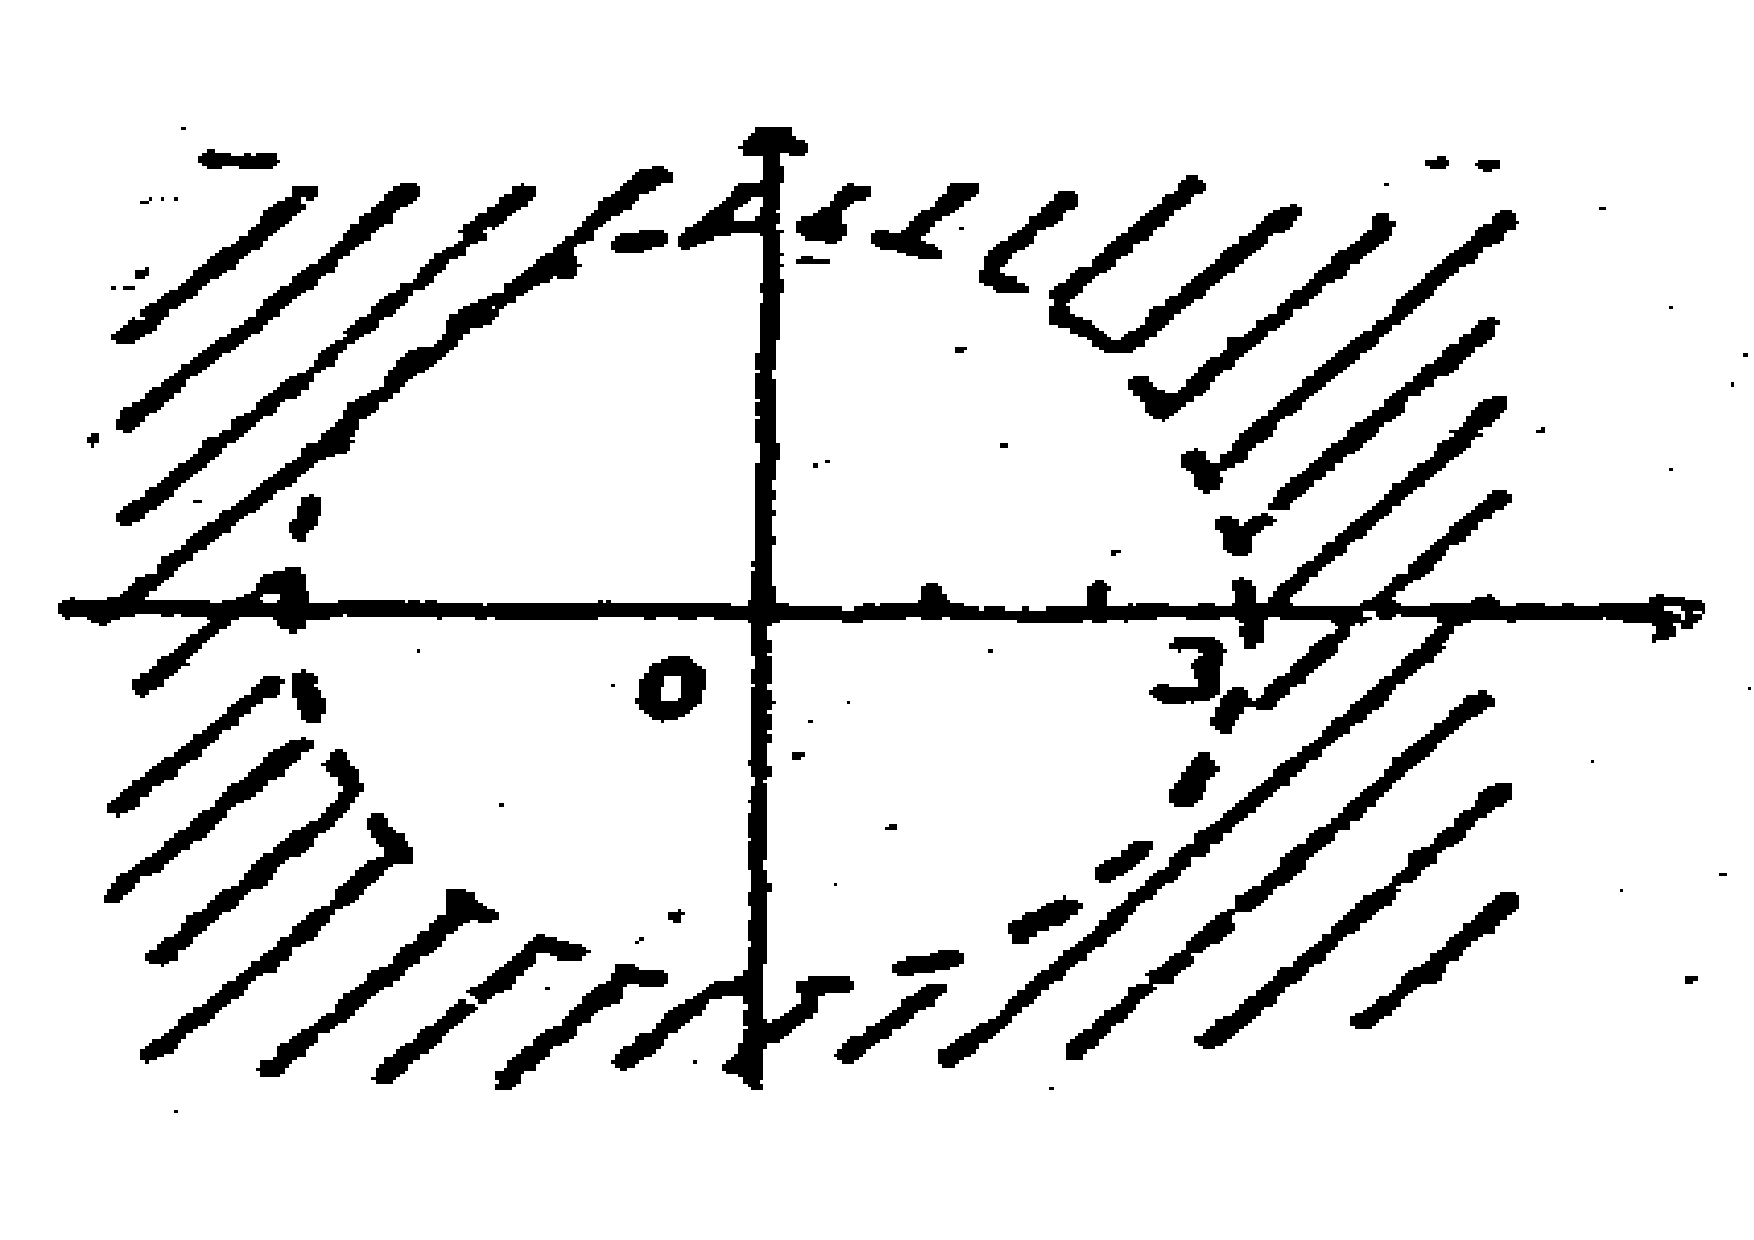
\includegraphics[width=0.45\textwidth]{images/b1p2-335-fig01}} b) \raisebox{-.5\height}		{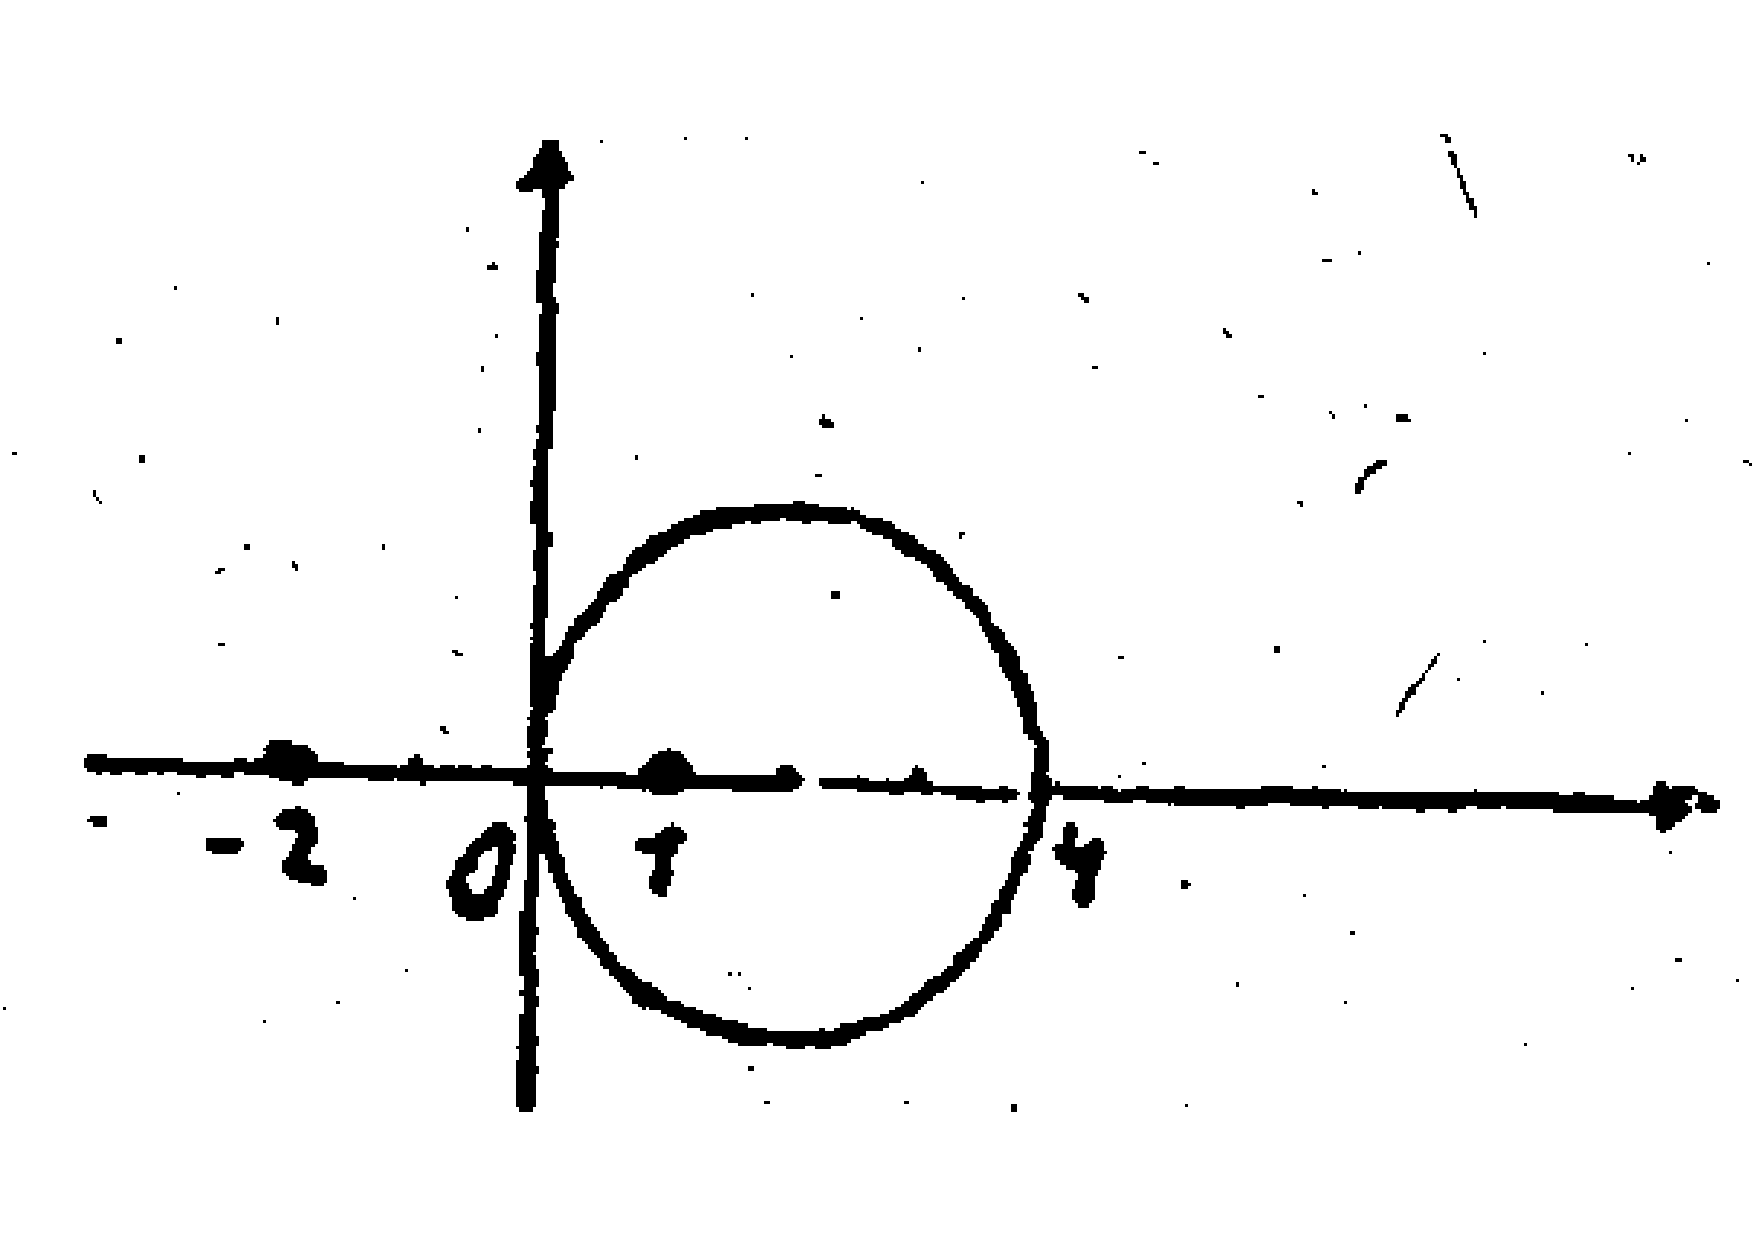
\includegraphics[width=0.45\textwidth]{images/b1p2-335-fig02}}

	\setcounter{enumi}{73}

	\item a) \raisebox{-.5\height}{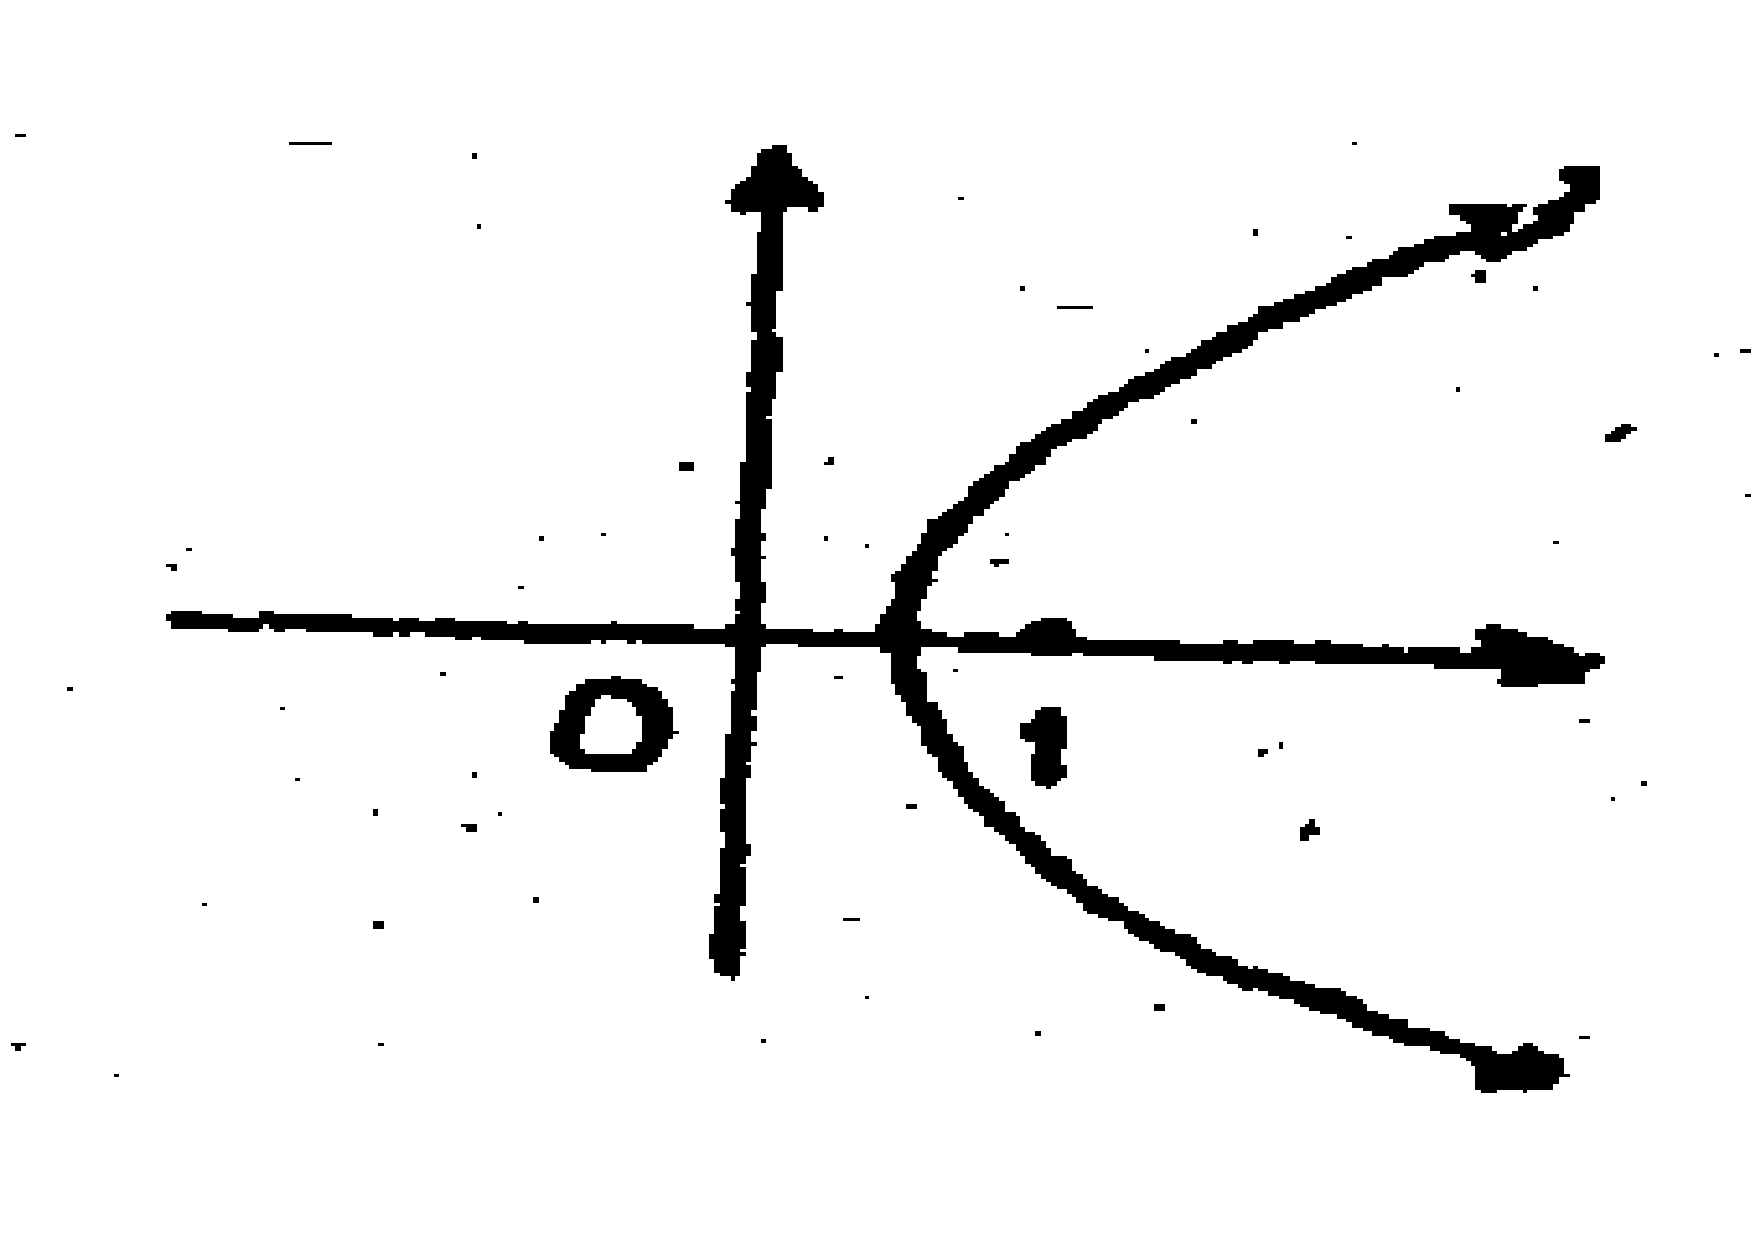
\includegraphics[width=0.45\textwidth]{images/b1p2-335-fig03}} b) \raisebox{-.5\height}{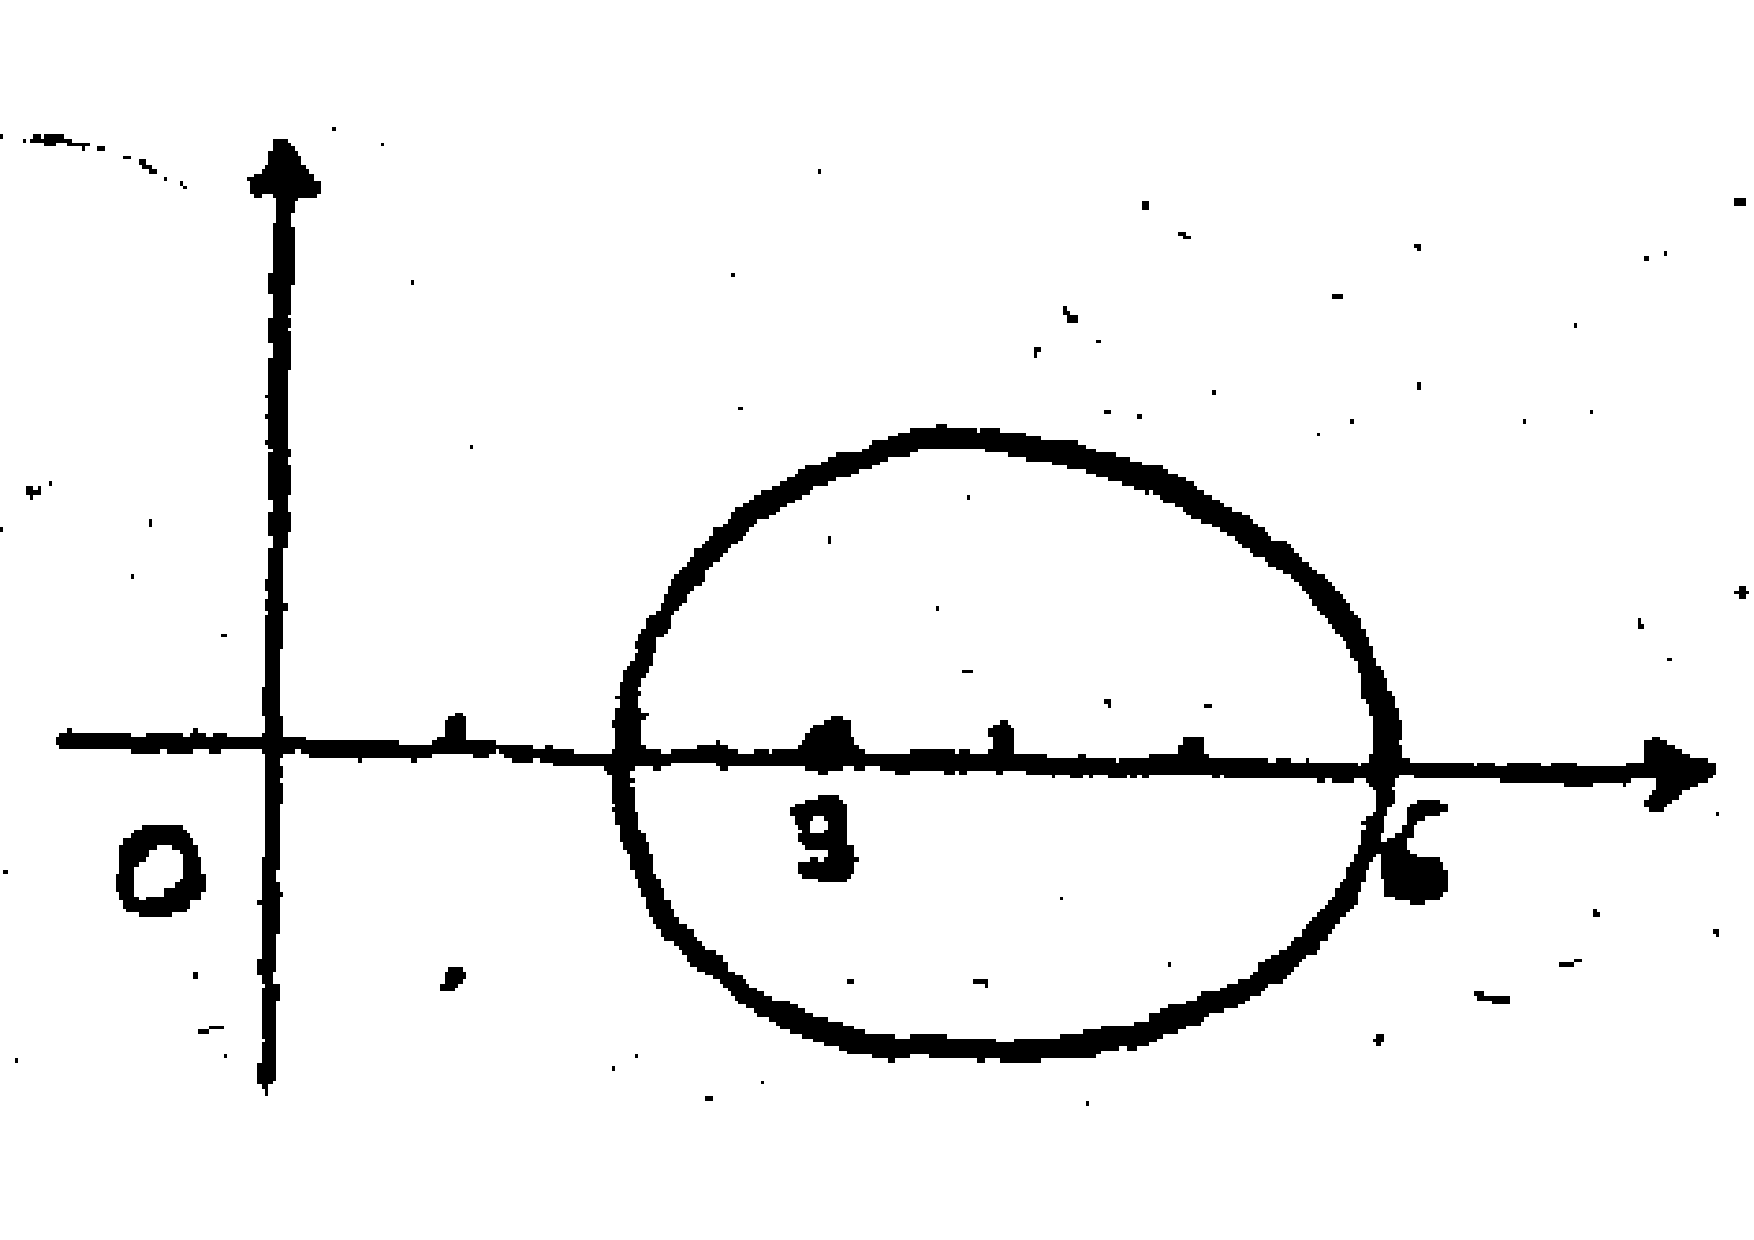
\includegraphics[width=0.45\textwidth]{images/b1p2-335-fig04}}

\end{enumerate}












% =======================================================
\end{document}  

%==== templates ====

%==== environments ====

%\begin{figure}[htb]
%	\centering
%	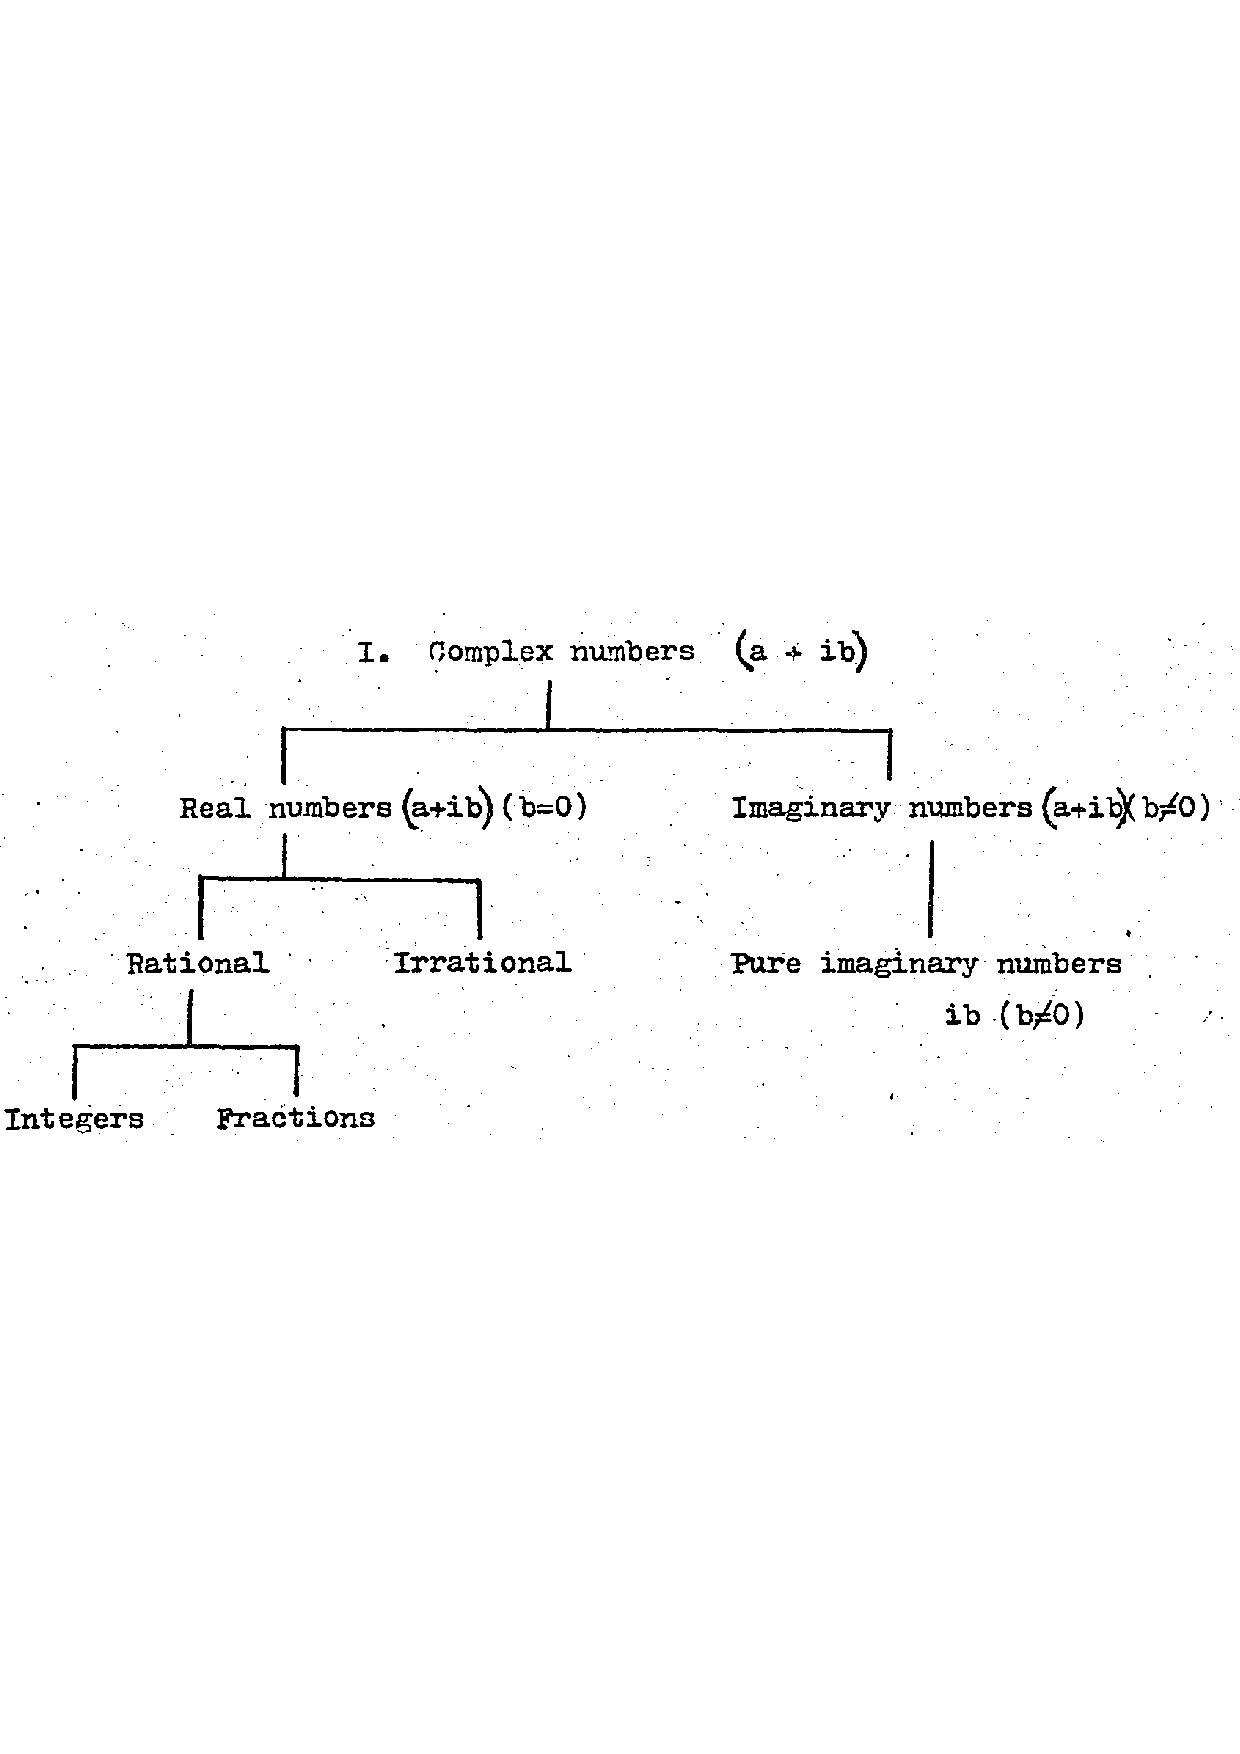
\includegraphics[width=0.9\textwidth]{images/SD-1-1p15A}
%	\caption{Classification of complex numbers}
%	\label{fig:classificationOfComplexNumbersA}
%\end{figure}

%\begin{center}
%\begin{tabular}{cc}
%\end{tabular}
%\end{center}

%\begin{exmp}
%\begin{hSolution}
%\end{hSolution}
%\end{exmp}

%\begin{hEnumerateAlpha}
%\end{hEnumerateAlpha}

%\begin{hEnumerateRoman}
%\end{hEnumerateRoman}

%$
%\begin{bmatrix}
%\end{bmatrix}
%$

%\frac{aaaa}{bbb}
%\frac{a_{n}}{b_{n}}
%\left( aaaa \right)
%\Longrightarrow

%\begin{multicols}{2}
%	bb
%\columnbreak
%	aa
%\end{multicols}
